\documentclass[12pt]{article}
% Reduce excessive hyphenation https://stackoverflow.com/a/65156105
\tolerance=9999
\emergencystretch=10pt
\hyphenpenalty=10000
\exhyphenpenalty=100

\usepackage[
top=1cm,
bottom=1cm,
left=1cm,
right=1cm,
headsep=6pt,
headheight=17pt, % as per the warning by fancyhdr
includehead,
heightrounded, % to avoid spurious underfull messages
]{geometry}
\usepackage{fancyhdr}
\newcommand{\smallerfont}{\fontsize{11}{13}\selectfont}
\fancypagestyle{plain}{%
  \fancyhf{}                      % Clear header and footer fields.
  \fancyhead[l]{\smallerfont{}Spring 2026}
  \fancyhead[c]{\smallerfont{}Syllabus: MSMI 3450: GPUs for Massively Parallel Mechanistic Modeling (3~credits)}
  \fancyhead[r]{\smallerfont{}Page \thepage{} of~\pageref*{mylastpage}}}
\pagestyle{plain}
\usepackage{graphicx}
\usepackage{sectsty}            % sectionfont
\sectionfont{\fontsize{12}{15}\selectfont}
\usepackage{soul}
\usepackage{hyperref}           % clickable links
\hypersetup{colorlinks=true,citecolor=blue,linkcolor=blue,urlcolor=blue}
\urlstyle{rm}
\usepackage[
abbreviate=true,
bibencoding=utf8,
minnames=2,
maxbibnames=99,
sorting=none,
style=vancouver,
citestyle=numeric-comp
]{biblatex}
% The vancouver citation style is based on NLM per
% https://tex.stackexchange.com/a/371433
\addbibresource{references.bib}
\usepackage{upgreek}                % \upalpha
% Highlight author.
\renewcommand*{\mkbibnamegiven}[1]{%
  \ifitemannotation{highlight}{\textbf{\color{red} #1}}{#1}}
\renewcommand*{\mkbibnamefamily}[1]{%
  \ifitemannotation{highlight}{\textbf{\color{red} #1}}{#1}}
% Bibliography text size.
\renewcommand*{\bibfont}{\footnotesize}

\begin{document}

% https://poorvucenter.yale.edu/teaching/teaching-resource-library/syllabus-design

\begin{description}
\item[Instructor] Pariksheet Nanda, PhD \quad %
  \href{mailto:pan79@pitt.edu}{pan79@pitt.edu} \quad %
  The Assembly \#3099 \quad %
  Mo, Tu 13:00--15:00
\end{description}

\section{Course description}

Graphical Processing Units (GPUs) %
are not just for artificial intelligence (AI) or %
video games!
%
\ul{GPUs now power the worlds fastest supercomputers %
to solve the most computationally difficult, %
mechanistic scientific problems} in %
physics, %
chemistry, %
biology, %
material sciences, %
energy, %
earth and space sciences, %
national security, %
data analytics, and %
optimization.
%
A 7~year, \$1.8~billion effort %
called the Exascale Computing Project %
involving 2,800 scientists and engineers %
recently finished modernizing %
the underlying scientific numerical software %
to efficiently use this new generation of machines %
at more than a billion, billion floating point calculations per second %
referred to as exaflops.
%
While the National Science Foundation (NSF) NAIRR %
and the computing facilities themselves directly grant %
U.S. institutional and industry researchers like you %
\ul{to use these machines for your research projects at no cost, %
you have to do the work showing that %
your computations efficiently use %
multiple GPUs across many computer servers, %
thus scaling to solve large computational problems}.
%
This class will teach you %
computational skills to program for data parallel architecture, %
statistical techniques to tune your model to match heterogeneous datasets, %
testing and feedback %
to regularly verify and improve your software quality, %
and you will solve a real-world research problem with your own faculty mentor.

This course is for undergraduate students, %
graduates students, %
faculty and staff---%
including those working with university research clusters and %
at the Pittsburgh Super Computing center.
%
\ul{Undergraduate students and staff members %
must e-mail the instructor a letter of support from a faculty mentor %
within the first 2 weeks of the course, %
ideally even before the course begins} %
for the instructor to help scope the capstone project %
and to group learners in complementary research areas together.
%
This course does not focus on AI tools---%
there are plenty of courses covering those---%
but instead focuses on high performance computing (HPC) tools %
and HPC numerical libraries %
that can be instrumented for hardware performance analysis.
%
The capstone project is intended to support %
summer NSF research experiences for undergraduates (REU), %
core-facility staff collaborations, %
and preliminary grant work of %
faculty, postdoctoral trainees, and graduate students.

\noindent
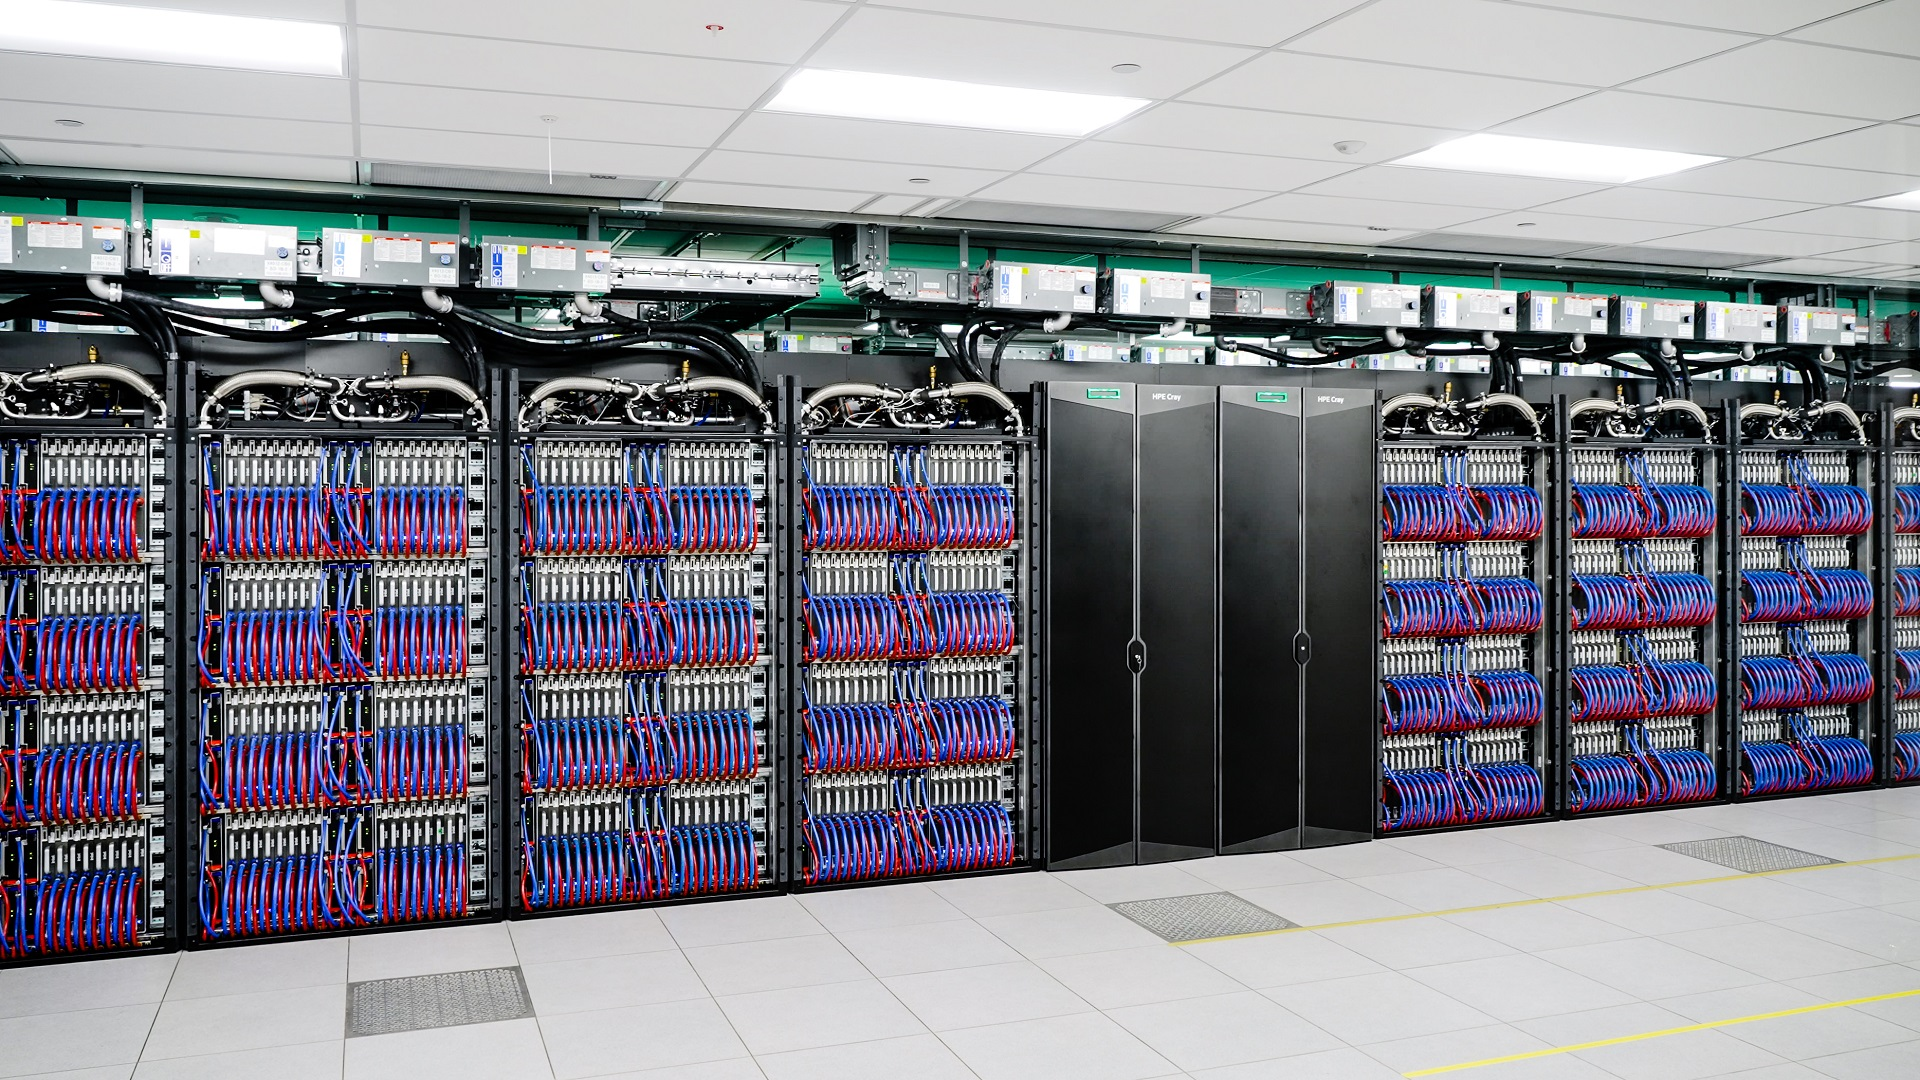
\includegraphics[width=\linewidth]{1920x1080-Aurora hero image.jpg}
% https://www.anl.gov/sites/www/files/2024-05/1920x1080-Aurora hero image.jpg
Photo: The Aurora supercomputer at Argonne National Laboratory; %
rank 3 in the Top 500 List of June 2025.

\section{Course prerequisites}

\begin{itemize}
\item Familiarity with at least one %
  procedural computer programming language %
  (such as C, C++, C\#, Fortran, Rust, Swift, %
  Python, R, Julia, GNU Octave, MATLAB, %
  Perl, Ruby, Java, Lisp, etc.)

  The class will use C++, Python, and a small amount of Bash shell scripting.
\item Basic statistical knowledge %
  of mean, median, standard deviation, and L2-norm.

  The class uses these statistical concepts to construct %
  summary functions for matching computational models with datasets; %
  they are also used in performance profiling tools.
\item Laptop computer to use in class running an operating system %
  supported for scientific processing and visualization software %
  such as GNU/Linux, macOS, or Windows %
  (namely, ChromeBooks, iPads, and smartphones would likely not be suitable).

  Typically, %
  GNU/Linux is best supported in scientific computing %
  and immersing yourself using that as your everyday machine %
  will support a career in this field; %
  several commercial vendors sell GNU/Linux laptops\footnote{%
  % US-based - only GNU/Linux.
  System76, ThinkPenguin, Purism, %
  % US-based - optional GNU/Linux.
  Framework, Malibal, %
  % International.
  NovaCustom, Tuxedo Computers, StarLabs, Slimbook, %
  % Refurbished.
  Technoethical, Vikings, Libiquity, etc.}.
  %
  For the purposes of this class, %
  a laptop GPU with compute capability\footnote{%
  Intel Xe (in Intel Arc GPUs), AMD ROCm, and Nvidia CUDA} %
  would allow you to develop and test code locally %
  instead of testing on remote machines.
\end{itemize}

\noindent
Please contact the instructor for a permission number to join the course.
% 
No software installation is necessary before the course begins.  

\section{Learning objectives}

\section{Required resources}

\section{Assessment}

\section{Course schedule}

\begin{enumerate}
\item Strategies for within-node vectorization, caching, memory bandwidth, and
  I/O
  \begin{itemize}
  \item Exercises vectorizing Python code, inspecting C assembler CPU
    vectorized instructions, creating roofline plots to inspect CPU-memory,
    hwloc to inspect memory CPU hierarchy
  \item Goal is appreciating the value of low-level computing
  \end{itemize}
\item Strategies for task distribution and multi-node cluster scaling
  \begin{itemize}
  \item Exercises with C, TaskWorks
    (\url{https://github.com/hpc-io/taskworks}), Spack, MPI, and SLURM
  \item Goal is reducing I/O overhead by batching and threading
  \end{itemize}
\item Introduction to data parallel programming for GPUs
  \begin{itemize}
  \item Exercise with C++ Kokkos
  \end{itemize}
\item Pseudo-likelihood based parallel parameter estimation
  \begin{itemize}
  \item Exercise with Python pyABC ABC-SMC
  \end{itemize}
\item Introduction to performance engineering
  \begin{itemize}
  \item Exercise with Darashan, Drishti
    (\url{https://github.com/hpc-io/drishti-io}), and HPCtoolkit
  \end{itemize}
\item Stress-free peer code review and testing
  \begin{itemize}
  \item Exercise with professor and pairing
  \end{itemize}
\item Capstone project; potential topics for students without existing,
  relevant research projects:
  \begin{itemize}
  \item Scaling up data science-centric workflows (with CharlieCloud)
  \item On-demand complexity at scale (with Apptainer, Galaxy, and )
  \item AI acceleration (with biologically-informed neural networks [BINNs])
  \end{itemize}
\end{enumerate}


\section{Academic integrity}

Students in this course %
will be expected to comply with %
the University of Pittsburgh's %
Policy on Academic Integrity%
\footnote{\url{https://www.provost.pitt.edu/info/ai1.html}}.
%
Any student suspected of violating this obligation %
for any reason during the semester %
will be required to participate in the procedural process, %
initiated at the instructor level, %
as outlined in the University Guidelines on Academic Integrity.
%
This may include, %
but is not limited to, %
the confiscation of the examination %
of any individual suspected of violating University Policy.
%
Furthermore, %
no student may bring any unauthorized materials to an exam, %
including dictionaries and programmable calculators.

To learn more about Academic Integrity, %
visit the Academic Integrity Guide%
\footnote{\url{http://pitt.libguides.com/academicintegrity/}} %
for an overview of the topic.
%
For hands-on practice, %
complete the Academic Integrity Modules%
\footnote{\url{http://pitt.libguides.com/academicintegrity/plagiarism}}.

\section{Disability services}

If you have a disability %
for which you are or may be requesting an accommodation, %
you are encouraged to contact %
both your instructor and Disability Resources and Services (DRS)%
\footnote{\url{https://www.studentaffairs.pitt.edu/drs/}}, %
140 William Pitt Union, %
(412)~648-7890, %
\href{mailto:drsrecep@pitt.edu}{drsrecep@pitt.edu}, %
(412)~228-5347 for P3 ASL users, %
as early as possible in the term.
%
DRS will verify your disability %
and determine reasonable accommodations for this course.

\label{mylastpage}              % chktex 24
\newpage
\appendix
\setcounter{page}{1}
\renewcommand{\thepage}{\arabic{page}}
\fancyhead[c]{References}
\fancyhead[r]{Appendix Page \thepage{} of~\pageref*{mylastappendixpage}}
\printbibliography[heading=none]{}%
\label{mylastappendixpage}

\end{document}
